\documentclass[14pt]{beamer}

\title{Goats and Tiger}
\subtitle{Team 11}

\author[]{S.Sai Harshitha \newline P.Pratyusha \newline G.Neha \newline K.Sri Tulasi \newline BH. Sai Shruthi \newline Chennupati Madhuri}

\date{March 22, 2021}

\usetheme{CambridgeUS}
\usecolortheme{dolphin}
\usepackage{graphicx}
\usepackage{grffile}

\begin{document}
\begin{frame}
	\titlepage
\end{frame}
\begin{frame}{What is Goats and Tiger?}
		Bagha Chal or Moving Tiger is an ancient Nepali board game.
\end{frame}

\begin{frame}{Structure of game board}
	3 Tigers and 15 goats
	\begin{center}
		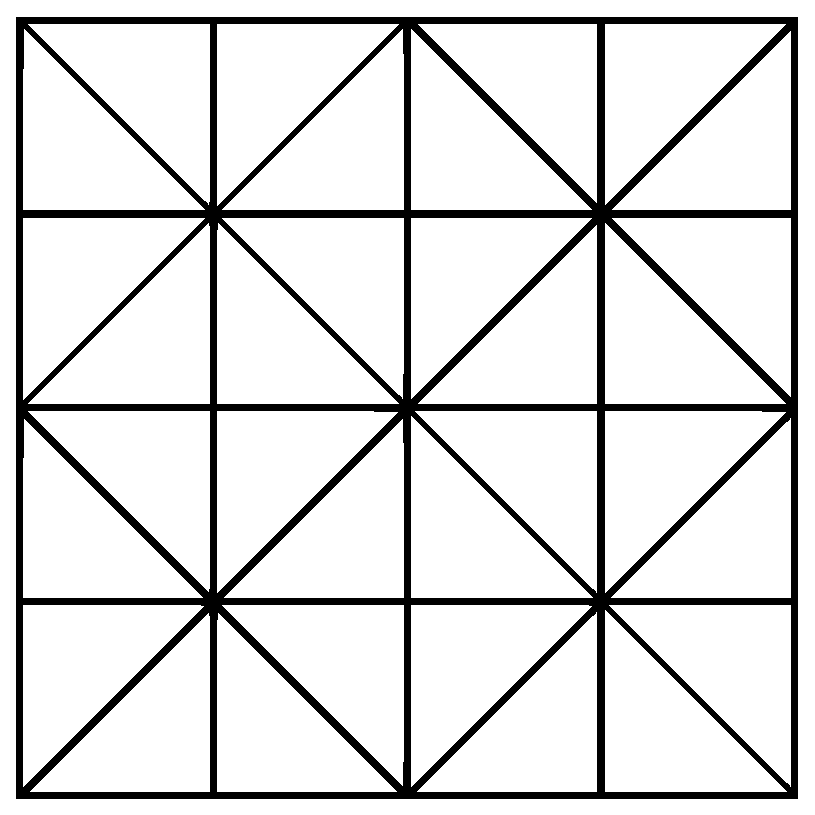
\includegraphics[width=5cm, height=5cm]{goatsTiger_conv.eps}
	\end{center}
\end{frame}

\begin{frame}{Tech Stack}
	\begin{itemize}
		\item Pygame
        	\item PyCharm
		\item Git
        	\item LaTeX
	\end{itemize}
\end{frame}

\begin{frame}{Workflow}
	\begin{itemize}
		\item Setup workspace
		\item Learn Pygame
		\item Collect resources
		\item Fix on the design
		\item Start coding
	\end{itemize}
\end{frame}

\begin{frame}
	\begin{center}
	\textbf{\huge Thank You!}
	\end{center}
\end{frame}

\end{document}
	

